\section{Momentum}
Momentum is an extremely important concept that will come up time and time again in all types of ways. Very simply put, momentum looks at how inert
something is and how fast its moving. There are translational and angular (rotational) momentums. We'll start by discussing the properties of momentum 
with reference to translational momentum. Just know all of these qualities apply to angular momentum except for the one special case about angular
momentum. The momentum equation is as follows.
\begin{equation}
    \vec{p} = m \vec{v}.
\end{equation}
The unit is $\frac{Kgm}{s}$ or more simply $Ns$.

\subsection{Conservation of Momentum}
In all collisions for this class, momentum is conserved. That means 
\begin{equation}
    \vec{p}_{Initial} = \vec{p}_{Final}.
\end{equation}
This will be an extremely useful concept moving forward.

\subsection{Types of Collisions}
There are two types of collisions that may occur. \textbf{Elastic} and \textbf{Inelastic} collisions. 

\subsubsection{Elastic Collisions}
Elastic collisions (visually) occur when two objects hit and bounce off. That's a good rule of thumb and will apply to most cases in this course, but
we can also be more precise. An \textbf{Elastic Collision} is any collision that conserved momentum and kinetic energy (we'll talk about kinetic energy
in the next section. For now, just understand that its some property being conserved). In math terms,
\begin{eqnarray*}
    \vec{p}_{Initial} = \vec{p}_{Final} \\
    K_{Initial} = K_{Final}
\end{eqnarray*}

Since kinetic energy is conserved, we can actually write a special equation that makes it easier to solve for velocities. This only applies to
\textbf{1D collisions}.
\begin{equation}
    v_1 + v_1^\prime = v_2 + v_2^\prime
\end{equation}
The prime represents the final velocity for object one or object two. This \textbf{DOES NOT} apply to angular momentum since by definition it doesn't
happen in one dimension.

\subsubsection{Inelastic Collisions}
A good rule of thumb for this type of collision is when two things hit each other and stick together. In an \textbf{Inelastic Collision}, momentum is
conserved, but kinetic energy is not. So,
\begin{eqnarray*}
    \vec{p}_{Initial} = \vec{p}_{Final} \\
    K_{Initial} \neq K_{Final}
\end{eqnarray*}

\subsection{Impulse and Newton's Second Law Revisited}
The change in momentum is an important concept. We call the change in momentum "impulse" and represent it with a $J$.
\begin{equation}
    \vec{J} = \Delta \vec{p}.
\end{equation}

Earlier, we defined Newton's Second Law as
\begin{eqnarray*}
    F = \frac{\text{d} \vec{p}}{\text{d}t}
\end{eqnarray*}
Now you know what the $p$ means.

\subsection{Angular Momentum}
We'll conclude this section by talking about \textbf{angular momentum}, which is how inert and how fast something is rotationally. We write it
using the following equation.
\begin{equation}
    \vec{L} = I \omega = \vec{r} \times \vec{p}
\end{equation}
Notice how the second iteration involves the cross product. The ideas of two types of collisions and whatnot still apply. However, again note the special
equation for elastic equations doesn't.

We can also use angular momentum to define net torque.
\begin{equation}
    \tau_{net} = \frac{\text{d} \vec{L}}{\text{d} t}
\end{equation}

\subsubsection{Angular Momentum of an Object Moving Linearly}
We can actually determine the angular momentum of an object moving in a straight line. Consider the image below.

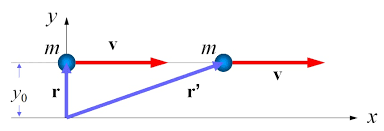
\includegraphics{linear_L.png}

First, we establish a "pivot" point. This is the point we are interested in the object's angular momentum around. We'll just have this be the
origin (where the two blue lines meet). To find the angular momentum in this case, we take the shortest distance between the path of the object
$r$. Then, just take the cross product with momentum (the second iteration of the angular momentum equation.)